\documentclass[11pt,letterpaper]{article}

% ── Packages ──────────────────────────────────────────────
\usepackage[margin=1in]{geometry}
\usepackage{amsmath,amssymb,amsthm}
\usepackage{mathtools}
\usepackage{booktabs}
\usepackage{enumitem}
\usepackage{hyperref}
\usepackage[dvipsnames]{xcolor}
\usepackage{titlesec}
\usepackage{microtype}
\usepackage{parskip}
\usepackage{tikz}
\usepackage{multicol}
\usetikzlibrary{arrows.meta,positioning,calc,fit,backgrounds}

% ── Formatting ────────────────────────────────────────────
\hypersetup{colorlinks=true, linkcolor=NavyBlue, citecolor=NavyBlue, urlcolor=NavyBlue}
\titleformat{\section}{\large\bfseries}{\thesection}{1em}{}
\titleformat{\subsection}{\normalsize\bfseries}{\thesubsection}{1em}{}
\titleformat{\subsubsection}{\normalsize\itshape}{\thesubsubsection}{1em}{}

% ── Custom environments ──────────────────────────────────
\newcommand{\caveat}[1]{\par\smallskip\noindent\textcolor{gray}{\textit{Caveat:} #1}\smallskip}
\newcommand{\assumption}[1]{\par\smallskip\noindent\textcolor{BrickRed}{\textit{Assumption:} #1}\smallskip}
\newcommand{\pp}{\,\text{pp}}

% ── Math shortcuts ────────────────────────────────────────
\newcommand{\bfp}{\mathbf{p}}
\newcommand{\bfz}{\mathbf{z}}
\newcommand{\bfy}{\mathbf{y}}
\newcommand{\bfd}{\mathbf{d}}
\newcommand{\bfb}{\mathbf{b}}
\newcommand{\cS}{\mathcal{S}}
\newcommand{\cM}{\mathcal{M}}
\newcommand{\R}{\mathbb{R}}

\begin{document}

% ── Title ─────────────────────────────────────────────────
\begin{center}
{\LARGE\bfseries Neural Field Perceiver}\\[6pt]
{\large Cross-Patient Speech Decoding from Intra-Operative $\mu$ECoG\\via Reprojection-Supervised Spatial Alignment}\\[12pt]
{\normalsize Ben Tang \quad\textbar\quad Greg Cogan Lab, Duke University}\\[4pt]
{\normalsize April 2026 \quad\textbar\quad Version 3}
\end{center}

\medskip\noindent\rule{\textwidth}{0.4pt}\medskip

\noindent This document is the complete technical reference for the Neural Field Perceiver project. It unifies the theoretical problem framing, cross-disciplinary foundations from 3D computer vision, the full architecture specification, uncertainty estimation, and the experimental plan. Claims throughout are categorized as \textbf{externally established} (published literature), \textbf{internally observed} (our experiments), or \textbf{working hypotheses} (plausible but unverified). Structural assumptions that could be wrong are marked in \textcolor{BrickRed}{red}.

\tableofcontents
\newpage


%% ====================================================================
%%  PART I: PROBLEM FRAMING
%% ====================================================================

\part{Problem Framing}

\section{The Physical Problem}

Each patient's micro-electrocorticography ($\mu$ECoG) array is a \textbf{sparse spatial sample} of neural activity over the cortical surface during speech production. The array is placed subdurally over left ventral sensorimotor cortex (vSMC) during surgery, and its position in standardized brain space (MNI-152) is determined post-hoc via electrode reconstruction (BioImage Suite for DBS patients, Brainlab for tumor patients).

\subsection{The cortical surface, not free 3D space}

The cortex is a folded two-dimensional sheet, not a volume. Let $\cS$ denote the cortical surface embedded in $\R^3$. The high-gamma analytic amplitude (HGA, 70--150\,Hz envelope) is a function on this surface:
\begin{equation}
a: \cS \times \R \to \R
\end{equation}

For patient $i$ with $N_i$ electrodes at cortical surface positions $\{\bfp_j^{(i)}\}_{j=1}^{N_i} \subset \cS$, we observe:
\begin{equation}\label{eq:observation}
\boxed{d_j^{(i)}(t) = a\bigl(\bfp_j^{(i)},\; t\bigr) + \epsilon_j^{(i)}(t)}
\end{equation}
where $\epsilon$ captures measurement noise, electrode impedance variation, and sub-electrode-scale neural activity not resolved by the ${\sim}2$\,mm contact spacing.

In practice, we approximate cortical surface positions with 3D MNI coordinates: $\bfp_j^{(i)} \approx (x_j^{(i)}, y_j^{(i)}, z_j^{(i)})_{\text{MNI}}$. This approximation has two consequences:

\begin{enumerate}[leftmargin=2em]
\item \textbf{Euclidean distance in MNI space does not equal geodesic distance on the cortical surface.} Two electrodes 3\,mm apart in MNI may sit on opposite banks of a sulcus, making them functionally distant. For $\mu$ECoG arrays on exposed cortex, the local patch under the array is approximately planar, so within-array Euclidean distances are reasonable. Cross-patient comparisons at larger scales are more affected by folding geometry.

\item \textbf{Surface-based coordinates} (e.g., projection to \texttt{fsaverage}) would better respect cortical geometry than volumetric MNI coordinates. Whether surface reconstructions exist for our patients depends on the BioImage Suite\,/\,Brainlab outputs available.
\end{enumerate}

\textbf{The decoding problem.} Given observations $\{d_j^{(i)}(t)\}$ at approximately known surface positions, infer the phoneme sequence $\bfy = (y_1, y_2, y_3)$ that produced the spatiotemporal pattern.

\textbf{The cross-patient problem.} Train on patients $\{1, \ldots, K\}$ and decode for a held-out patient $K{+}1$ whose electrodes sample the cortical surface at \emph{different positions}. The observations are not aligned: electrode $j$ on patient $i$ and electrode $j$ on patient $i'$ correspond to different cortical locations.

\subsection{What makes this hard}

\begin{table}[h]
\centering\small
\begin{tabular}{@{}lll@{}}
\toprule
\textbf{Factor} & \textbf{Quantity} & \textbf{Implication} \\
\midrule
Electrodes per patient & 63--201 & Sparse sampling of the cortical field \\
Electrode spacing & ${\sim}2$\,mm & Resolves individual gyral columns \\
Array offset across patients & 15--25\,mm in MNI & Different cortical regions sampled \\
Array rotation & Variable & Channel indices meaningless across patients \\
Correspondence uncertainty & Several mm & Coordinate-based alignment is approximate \\
Cortical folding variability & Patient-specific & Sulcal geometry differs across individuals \\
Tumor mass effect (subset) & Variable & Macroscopic warping in 6 of 12 patients \\
Trials per patient & 46--178 & Small-data regime for supervised learning \\
Total utterance per patient & ${\sim}1$\,min & Insufficient for single-patient SSL \\
Phoneme vocabulary & 9 classes $\times$ 3 positions & 27-way classification at each trial \\
\bottomrule
\end{tabular}
\end{table}


\section{The Shared Dynamics Hypothesis}

Cross-patient decoding is only possible if the cortical field $a(\bfp, t)$ shares structure across patients. We decompose:
\begin{equation}\label{eq:decomposition}
\boxed{a^{(i)}(\bfp, t) = f\bigl(T_i(\bfp),\; t;\; \bfy\bigr) + r^{(i)}(\bfp, t)}
\end{equation}
where:
\begin{itemize}[leftmargin=2em]
\item $f(\cdot, t; \bfy)$ is the \textbf{shared neural field}---the spatiotemporal pattern that phoneme sequence $\bfy$ produces in canonical cortical space.
\item $T_i: \cS_i \to \cS_{\text{canonical}}$ is a \textbf{patient-specific spatial transform} mapping each patient's cortical surface to a canonical reference. MNI normalization is our estimate of $T_i$, but it is imperfect.
\item $r^{(i)}(\bfp, t)$ is a \textbf{patient-specific residual} capturing individual neural organization, signal characteristics, and functional plasticity.
\end{itemize}
The viability of cross-patient decoding depends on the ratio $\|f\| / \|r^{(i)}\|$ at the spatial resolution accessible to our measurements and alignment procedure.

\subsection{Evidence for shared dynamics}

\subsubsection{Externally established (published literature)}

\textbf{Per-patient input layers + shared temporal backbone is the optimal transfer architecture.} Singh et al.\ (2025) demonstrate group training with $N{=}25$ sEEG patients: per-patient Conv1D + shared BiLSTM ($2{\times}64$), frozen shared backbone + fine-tuned per-patient layers yields PER 0.49 vs.\ 0.57 single-subject ($p{<}0.001$). Willett et al.\ (2023) use per-day affine input layer ($256{\to}256$) + shared 5-layer GRU (512 hidden) for day-to-day BCI transfer.

\caveat{Singh's data regime is ${\sim}60$\,min/patient (vs.\ our ${\sim}1$\,min); Conv1D hyperparameters are unreported. Willett is $N{=}1$ with ${\sim}40$\,min/day. The architectural pattern transfers; the hyperparameters do not.}

\textbf{Articulatory somatotopy in vSMC is reproducible within individuals.} Metzger et al.\ (2023) show somatotopic organization of speech articulators in one patient with chronic ECoG (253 channels): labial, front tongue, back tongue, and vocalic representations are spatially organized ($p{<}0.0001$), preserved even after 18 years of anarthria.

\caveat{$N{=}1$ chronic implant. Cross-patient spatial consistency is inferred from anatomical uniformity but not directly measured in any paper in our corpus.}

\textbf{Articulatory features are a robust encoding basis in vSMC.} Wu et al.\ (2025) reconstruct speaker-invariant articulatory features from HD-ECoG over vSMC (PCC 0.75--0.80, $N{=}3$), including one intra-operative patient (PCC\,=\,0.76).

\textbf{MNI coordinates enable cross-patient ECoG transfer.} Chen et al.\ (2025, SwinTW) use MNI coordinates and ROI embeddings across 43 ECoG + 9 sEEG subjects, reporting mean PCC\,=\,0.765 on unseen participants in cross-validation.

\caveat{Standard ECoG has ${\sim}10$\,mm spacing, comparable to inter-subject correspondence uncertainty. Our $\mu$ECoG spacing (${\sim}2$\,mm) is finer, meaning coordinates may encode global array position but not resolve within-array relationships.}

\textbf{Motor cortex neural manifold structure is preserved across individuals.} Safaie et al.\ (2023, \textit{Nature Neuroscience}) show motor cortex population dynamics during reaching are geometrically similar across monkeys. Gallego et al.\ (2020, \textit{Nature Neuroscience}) show low-dimensional manifold dynamics are preserved within individuals across time despite neural turnover.

\caveat{Safaie: limb motor cortex, non-human primates. Gallego: within-individual. Extension to cross-individual speech motor cortex is plausible but untested.}

\textbf{Consistent articulatory somatotopy across participants.} Bouchard et al.\ (2013, \textit{Nature}) demonstrated reproducible articulatory maps in vSMC across 3 participants. Anumanchipalli et al.\ (2019, \textit{Nature}) reconstructed continuous articulatory trajectories from motor cortex.

\subsubsection{Internally observed (our experiments)}

\textbf{Cross-patient supervised transfer works at this data scale.} Our LOPO pipeline achieves PER\,=\,0.762 on held-out S14, compared to per-patient PER\,=\,0.737 (grouped-by-token CV). Direct evidence that decodable shared structure exists in~$f$.

\textbf{Articulatory bottleneck head improves LOPO decoding.} Consistent with $f$ being organized along articulatory feature dimensions.

\textbf{55 experiments on S14 converge to PER 0.750--0.780.} See Section~\ref{sec:wall} for interpretation.

\textbf{SSL features carry partial structure.} JEPA + LP-FT achieves PER\,=\,0.797 (vs.\ 0.854 basic). Supervised features with the same recipe achieve 0.737.

\subsubsection{Working hypotheses (plausible but unverified)}

The ${\sim}0.76$ PER convergence partly reflects spatial alignment limitations (not isolated from data scarcity or S14-specific effects). MNI coordinates will improve decoding (depends on registration accuracy and whether alignment is binding). Cross-task data pooling (Duraivel 2025) is a high-value, low-risk path to more data.


\section{The Neural Manifold Connection}\label{sec:manifold}

\subsection{Two views of the same phenomenon}

The cortical field model and the neural manifold hypothesis are dual descriptions. The bridge is the \textbf{latent articulatory state} $\bfz(t) \in \R^k$:
\begin{equation}\label{eq:obs-function}
\boxed{d_j^{(i)}(t) = g\bigl(\bfp_j^{(i)},\; \bfz(t)\bigr) + \epsilon_j^{(i)}(t)}
\end{equation}
where $g: \cS \times \R^k \to \R$ is a \textbf{shared observation function}---the somatotopic map. The dynamics on the manifold are phoneme-determined:
\begin{equation}\label{eq:dynamics}
\dot{\bfz}(t) = h\bigl(\bfz(t);\; \bfy\bigr)
\end{equation}

\subsection{The factorization is the key insight}

The shared field $f(\bfp, t; \bfy)$ factorizes as $g(\bfp, \bfz(t))$, separating space from time through a low-dimensional bottleneck. The model learns:
\begin{enumerate}[leftmargin=2em]
\item A spatial function $g$: how each brain position encodes articulatory features (somatotopic map).
\item A dynamical system $h$: how the articulatory state evolves during speech.
\end{enumerate}

\subsection{Articulatory manifold dimensionality}

\begin{table}[h]
\centering\small
\begin{tabular}{@{}llc@{}}
\toprule
\textbf{Contrast} & \textbf{Phonemes distinguished} & \textbf{Dim.} \\
\midrule
Place of articulation & labial (b,p,v) vs.\ velar (g,k) & ${\sim}2$ \\
Manner & stop vs.\ fricative vs.\ vowel & ${\sim}2$ \\
Voicing & voiced (b,g,v) vs.\ voiceless (k,p) & ${\sim}1$ \\
Vowel height & low (a,\ae) vs.\ high (i,u) & ${\sim}1$ \\
Vowel backness & front (\ae,i) vs.\ back (a,u) & ${\sim}1$ \\
\midrule
\textbf{Effective dimension} & & $\mathbf{{\sim}5\text{--}8}$ \\
\bottomrule
\end{tabular}
\end{table}

\noindent Far below electrode count (63--201): the decoding problem is well-posed.

\subsection{Cross-patient transfer as manifold alignment}

Each patient's array gives a different projection: $\bfd^{(i)}(t) \approx W^{(i)} \bfz(t) + \boldsymbol{\epsilon}^{(i)}$, where $W^{(i)} \in \R^{N_i \times k}$ is determined by electrode positions. MNI coordinates provide the geometric relationship between projections a priori, rather than requiring post-hoc alignment (CCA, Procrustes, CORAL---all failed in our experiments).


\section{Decomposing Cross-Patient Variation}

\subsection{The spatial transform $T_i$}

\begin{equation}\label{eq:transform}
T_i(\bfp) = A_i \cdot \bfp + \bfb_i + \delta_i(\bfp)
\end{equation}
\begin{itemize}[leftmargin=2em]
\item $A_i \in \R^{3 \times 3}$: rigid or affine (rotation, scaling). MNI normalization estimates this.
\item $\bfb_i \in \R^3$: translation (15--25\,mm array placement offset).
\item $\delta_i(\bfp)$: nonlinear residual---sulcal geometry, local folding, \textbf{tumor mass effect} (geometric mapping error in 6/12 patients).
\end{itemize}

\subsection{Inter-subject correspondence uncertainty}

Not a fixed constant. Sources: native-space localization (sub-mm), brain shift correction (variable), atlas warping (dominant). Net: several mm for healthy anatomy, more near tumors.
\begin{itemize}[leftmargin=2em]
\item At somatotopy scale (${\sim}15$--$20$\,mm): reliable.
\item At electrode spacing (${\sim}2$\,mm): unreliable.
\item In between (${\sim}5$--$10$\,mm): partially informative.
\end{itemize}

\subsection{Resolution mismatch implies dual spatial encoding}

\begin{table}[h]
\centering\small
\begin{tabular}{@{}llll@{}}
\toprule
\textbf{Scale} & \textbf{Resolution} & \textbf{Best encoded by} & \textbf{What it captures} \\
\midrule
Cross-patient & ${\sim}10$--$15$\,mm & MNI coordinates & Articulatory somatotopy \\
Intra-patient local & ${\sim}2$\,mm & Grid topology & Fine-grained spatial patterns \\
\bottomrule
\end{tabular}
\end{table}

\subsection{The patient-specific residual $r^{(i)}$}

Captures: (1)~fine-grained neural organization varying across individuals; (2)~signal characteristics (impedance, contact, SNR); (3)~functional plasticity (accent, articulatory habits); (4)~pathology-specific effects (Parkinson's excitability changes, tumor-adjacent reorganization).


\section{What Our Experiments Reveal}

\subsection{The evaluation recipe dominates at this data scale}

\begin{table}[h]
\centering\small
\begin{tabular}{@{}llr@{}}
\toprule
\textbf{Component} & \textbf{Category} & \textbf{PER improvement} \\
\midrule
Label smoothing 0.1 & Training & $-4.1\pp$ \\
Mixup $\alpha{=}0.2$ & Training & $-1.7\pp$ \\
Per-position heads + dropout & Training & $-1.2\pp$ \\
\midrule
Weighted $k$-NN ($k{=}10$, cosine) & Evaluation & $-2.1\pp$ \\
TTA (16 augmented copies) & Evaluation & $-1.4\pp$ \\
Articulatory + CE dual head & Evaluation & $-1.1\pp$ \\
Best-of per fold & Evaluation & $-1.8\pp$ \\
\bottomrule
\end{tabular}
\end{table}

\noindent Backbone already extracts most signal; the bottleneck is extracting predictions from the representation.

\subsection{Multi-scale temporal structure is validated}

Multi-scale temporal encoding (stride 3+5+10) was the single best architectural improvement (PER $0.766 \to 0.750$). The three scales correspond to fast transitions (${\sim}15$\,ms), syllable dynamics (${\sim}25$\,ms), and phoneme-level patterns (${\sim}50$\,ms).

\caveat{Validated with the current BiGRU backbone. Optimal stride values may differ for the transformer temporal encoder proposed here; re-validation is needed (Section~\ref{sec:temporal}).}

\subsection{SSL features carry partial structure}

All SSL methods produce near-chance PER (0.85--0.91) under basic evaluation. JEPA + LP-FT achieves 0.797. SSL features are non-trivial but far weaker than supervised features.

\subsection{The ${\sim}$0.76 PER convergence on S14}\label{sec:wall}

55 experiments converge to PER 0.750--0.780. \textbf{Attributing this to any single bottleneck would be premature}:
\begin{enumerate}[leftmargin=2em]
\item \textbf{S14 is no longer held-out.} 55+ architectures evaluated $\Rightarrow$ it functions as a validation set.
\item \textbf{Measurement noise.} ${\sim}30$ samples per fold $\Rightarrow$ ${\pm}0.05$ PER noise. Differences ${<}2\pp$ are within noise.
\item \textbf{Target-data scarcity.} S14 has 153 trials. Stage~2 contributes only ${\sim}1.6\pp$.
\item \textbf{Spatial alignment may be one factor.} Not isolated as \emph{the} bottleneck.
\end{enumerate}


\section{The Case for MNI Coordinates}

\subsection{Currently unused information}

The current pipeline uses per-patient Conv2d on grid topology. Each Conv2d is independent. The model has \textbf{zero information} about cross-patient spatial relationships. The shared backbone implicitly assumes feature alignment across patients---anatomically false for independent per-patient encoders.

\subsection{What coordinates enable}

Knowing $\bfp_j^{(i)}$ allows learning $g$ as a shared function. Concretely: (1)~identifying which articulatory zone each electrode samples; (2)~sharing representations across patients at similar positions; (3)~contextualizing variable coverage.

\subsection{What coordinates do NOT guarantee}

Coordinates help only if correspondence uncertainty is small enough relative to somatotopic scale, the architecture exploits them, and spatial alignment is actually binding. \textbf{Their value must be demonstrated empirically.}


%% ====================================================================
%%  PART II: CROSS-DISCIPLINARY FOUNDATIONS
%% ====================================================================

\part{Cross-Disciplinary Foundations}

\section{The Multi-View Reconstruction Analogy}\label{sec:analogy}

Inspired by holistic performance capture (Hewitt et al., 2024), the cross-patient decoding problem maps to \textbf{fitting a parametric 3D model to 2D observations from multiple viewpoints}.

\subsection{The pose estimation mapping}

\begin{table}[h]\centering\small
\begin{tabular}{@{}p{0.42\textwidth}p{0.02\textwidth}p{0.48\textwidth}@{}}
\toprule
\textbf{3D Pose Estimation} & & \textbf{Neural Field Decoding} \\
\midrule
3D body model (SMPL mesh) & $\leftrightarrow$ & Shared neural field $g(\bfp, \bfz)$ on cortex \\[3pt]
Pose parameters $\theta$ & $\leftrightarrow$ & Articulatory state $\bfz(t)$ \\[3pt]
Shape parameters $\beta$ & $\leftrightarrow$ & Patient embedding $e^{(i)}$ \\[3pt]
Camera extrinsics $[R \mid t]$ & $\leftrightarrow$ & MNI offset $\Delta^{(i)}$ (+ optional $\omega^{(i)}$) \\[3pt]
Camera intrinsics $K$ & $\leftrightarrow$ & Per-patient gain/bias \\[3pt]
2D keypoints $x_j$ & $\leftrightarrow$ & Electrode observations $d_j^{(i)}(t)$ \\[3pt]
Projection function $\pi(\cdot)$ & $\leftrightarrow$ & Observation function $g(\cdot)$ \\[3pt]
\textbf{Reprojection loss} $\|\pi(V) - x\|^2$ & $\leftrightarrow$ & \textbf{Reprojection loss} $\|g(\bfp{+}\Delta, \hat{\bfz}) - d\|^2$ \\
\bottomrule
\end{tabular}
\end{table}

\subsection{What the analogy reveals}

\textbf{Why previous methods failed:} CCA/Procrustes/CORAL align 2D feature statistics---works for similar viewpoints, fails for 15--25\,mm offsets. Per-patient SpatialConv is a separate 3D model per camera---no sharing. Our approach is Structure from Motion: jointly estimate shared structure and all camera parameters.

\textbf{Why reprojection loss beats arbitrary SSL:} JEPA/VICReg/masked reconstruction used physically meaningless targets. Reprojection is geometrically grounded: ``if your latent estimate is correct, you should predict what every electrode observes.'' Self-supervised but geometrically constrained.

\subsection{Where the analogy breaks}\label{sec:disanalogies}

The mapping is structural, not exact. Three important disanalogies:

\begin{enumerate}[leftmargin=2em]
\item \textbf{Each patient is a different ``scene,'' not a different camera on the same scene.} In multi-view reconstruction, all cameras observe the SAME 3D scene simultaneously. Our patients are observed independently, at different times, producing different spatiotemporal patterns due to $r^{(i)}$. The shared structure $f$ exists but is weaker than multi-view photometric consistency. The reprojection loss is therefore noisier---it must reconstruct through patient-specific residual, not just geometric projection.

\item \textbf{Reprojection is electrode-sparse, not pixel-dense.} A $256{\times}256$ image provides 65K reprojection constraints per view. Our 63--201 electrodes provide 100--1000$\times$ fewer constraints per frame. The reprojection signal per frame is thin; it aggregates value primarily across the temporal dimension ($T {\approx} 200$ frames/trial $\times$ 1315 trials).

\item \textbf{The ``scene'' changes every frame.} In static reconstruction, the scene is fixed across views. Here, $\bfz(t)$ changes continuously, so each frame is a different scene for reprojection. This is closer to \textbf{dynamic NeRF}---but the temporal structure is phoneme-specific and short-lived (${\sim}1$\,s trials), not a persistent evolving scene.
\end{enumerate}

\noindent These disanalogies mean: the reprojection loss will be noisier and less constraining than its vision analog; geometric inductive biases (distance bias, bilinear factorization) must compensate; and the reprojection loss is a useful regularizer but \textbf{should not be expected to carry the architecture} the way photometric loss carries NeRF. The supervised classification loss remains primary.


\section{Validated Patterns from 3D Vision (2024--2026)}

\subsection{The field's trajectory: per-scene $\to$ feed-forward $\to$ foundation model}

Our architecture sits at step 2. Key transferable patterns:

\textbf{VGGT} (CVPR 2025 Best Paper): joint 3D attribute prediction from variable-length views. Validates Perceiver jointly estimating latent state + alignment.

\textbf{LVSM} (ICLR 2025 Oral): encoder-decoder with fixed latent tokens vs.\ decoder-only. Decoder-only wins with enough data; explicit structure wins at small scale. \textit{Validates our structured approach for ${\sim}1300$ trials.}

\textbf{MMGN} (ICLR 2024): continuous field reconstruction from sparse, irregularly sampled sensors using factorized spatiotemporal basis. \textbf{Most directly relevant.} Our bilinear decoder is structurally identical.

\textbf{SPARF} (CVPR 2023): NeRF from sparse and noisy poses. Directly analogous: our MNI coordinates are noisy poses; our electrodes are sparse views.

\textbf{Senseiver} (\textit{Nature Machine Intelligence} 2023): Perceiver IO for field reconstruction from sparse sensors---structurally identical to our spatial encoder.

\subsection{Architectural pattern validation}

\begin{table}[h]\centering\small
\begin{tabular}{@{}p{0.38\textwidth}p{0.56\textwidth}@{}}
\toprule
\textbf{Our component} & \textbf{Same pattern in vision} \\
\midrule
Perceiver cross-attention (virtual $\to$ actual) & Canonical-to-observation tokens (LRM, LVSM) \\
Virtual electrodes at learnable positions & Triplane NeRF / fixed latent tokens \\
MNI distance-biased attention & Geometry-aware attention (GraphSplat, MVSplat) \\
Bilinear decoder $\hat{d} = \phi(\bfp)^\top\psi(s)$ & Spatiotemporal factorization (MMGN) \\
Reprojection loss & Photometric loss (all NeRF/3DGS) \\
Learnable per-patient $\Delta$ & Learnable camera extrinsics (SPARF, AnySplat) \\
Patient embedding $e^{(i)}$ & Per-scene latent code (CodeNeRF) \\
Electrode masking & View dropout / masked pretraining (MAE) \\
Structured inductive bias for small data & Explicit geometry at small scale (LVSM) \\
\bottomrule
\end{tabular}
\end{table}

\subsection{What we are correctly NOT doing}

Diffusion priors (need millions of scenes), 4D Gaussian primitives (trials are independent events), foundation model scale (1300 trials cannot support ${>}200$K params), decoder-only architecture (needs massive data), contrastive SSL (failed in our experiments).

\subsection{The data scale gap}

\begin{table}[h]\centering\small
\begin{tabular}{@{}lll@{}}
\toprule
& \textbf{3D Vision} & \textbf{Our Problem} \\
\midrule
Training scenes/patients & 50K--1M+ & ${\sim}20$ patients \\
Observations per scene & 10--100+ images (M pixels) & 63--201 electrodes \\
Total data & TB scale & ${\sim}240$\,MB \\
Parameter budget & 50M--500M+ & ${\sim}200$K \\
\bottomrule
\end{tabular}
\end{table}

\noindent This gap means: we \textbf{must} use strong geometric inductive biases; the reprojection loss is valuable but electrode-sparse (Section~\ref{sec:disanalogies}); and our ${\sim}200$K architecture is correctly small. The field's finding that explicit geometric structure helps at small scale (LVSM, SPARF) directly validates our design.


\section{Uncertainty Estimation}\label{sec:uncertainty}

\subsection{From binary to continuous confidence}

The current pipeline has a binary mechanism: significant channel selection (keep/drop). Proper uncertainty replaces this with continuous per-electrode confidence.

\subsection{Two types of uncertainty}

\textbf{Aleatoric} (irreducible): ``This electrode is inherently noisy.'' Per-electrode, does not decrease with more data.

\textbf{Epistemic} (reducible): ``We lack data in this cortical region.'' Per-position, decreases with more patients.

\subsection{Recommended uncertainty stack}

\subsubsection{Tier 1: Minimal implementation, high value}

\textbf{Beta-NLL loss} (Seitzer et al., ICLR 2022). Replace MSE reprojection with learned per-electrode variance:
\begin{equation}
\mathcal{L}_{\text{reproj}}^{\text{UQ}} = \frac{1}{2}\Bigl(\log \hat{\sigma}_j^2 + \frac{(d_j - \hat{d}_j)^2}{\hat{\sigma}_j^2}\Bigr) \cdot \bigl(\hat{\sigma}_j^2\bigr)^{0.5}_{\text{sg}}
\end{equation}
\textbf{Scope}: Beta-NLL affects the \textbf{training loss only}---it downweights reprojection gradients from noisy electrodes, preventing them from distorting the encoder. It does \textbf{not} directly modulate attention weights at inference time.

\textbf{Learned confidence gate} (for inference-time uncertainty weighting). To propagate aleatoric uncertainty into the Perceiver attention, we add a lightweight per-electrode confidence scalar:
\begin{equation}
c_j = \sigma\bigl(\text{Linear}(\text{token}_j)\bigr) \in (0, 1)
\end{equation}
The confidence scales the attention \textbf{values} (not logits): $V_j \leftarrow c_j \cdot V_j$ before aggregation. High-impedance or low-SNR electrodes learn $c_j \approx 0$. This is architecturally separate from Beta-NLL and adds $d{+}1 = 65$ parameters.

\textbf{MC Dropout at inference} (Gal \& Ghahramani 2016). Keep dropout active, 10--20 passes, variance $=$ epistemic uncertainty. Remove dropout from output layer.

\textbf{Conformal prediction} (Angelopoulos \& Bates 2021). Post-hoc prediction \textbf{sets} with coverage guarantees. Use CV fold as calibration. Clinical value: ``model thinks /b/ or /p/ (both labial stops).''

\subsubsection{Tier 2: Moderate implementation}

\textbf{Evidential regression} (NIG prior): single-pass decomposed aleatoric + epistemic per electrode. \textbf{Probabilistic virtual electrodes} (pixelSplat-style): predict latent distributions, uncertainty propagates through the pipeline.

\subsection{How uncertainty actually connects to the architecture}\label{sec:uq-flow}

\begin{center}
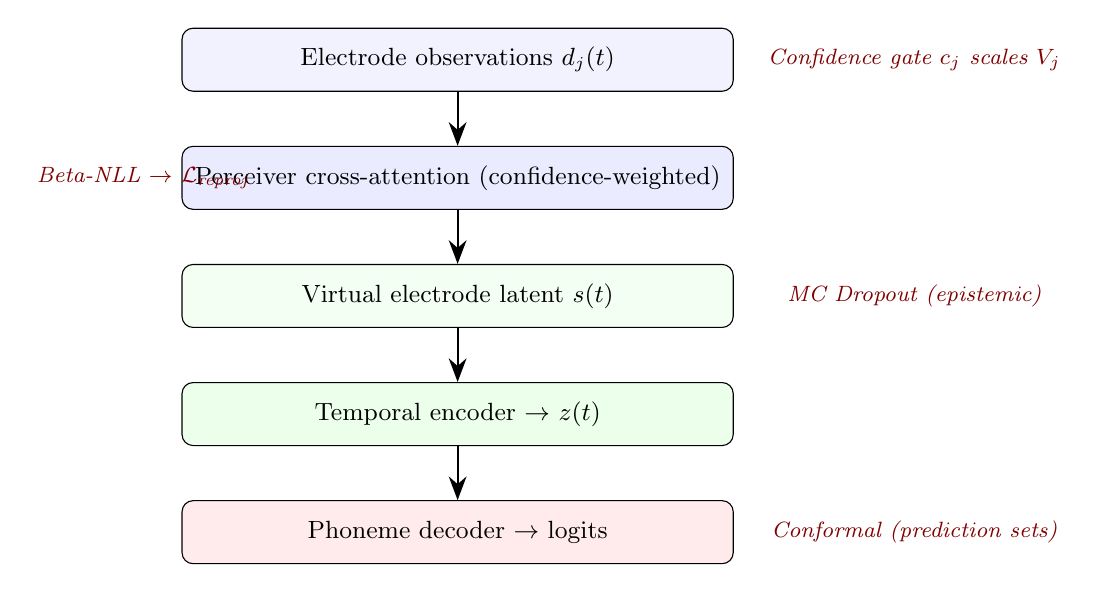
\begin{tikzpicture}[
  box/.style={draw, rounded corners, minimum width=7cm, minimum height=0.8cm, align=center, font=\small},
  uq/.style={font=\footnotesize\itshape, text=Maroon},
  arrow/.style={-{Stealth[length=3mm]}, thick}
]

\node[box, fill=blue!5] (elec) at (0, 0) {Electrode observations $d_j(t)$};
\node[uq] (uq1) at (5.8, 0) {Confidence gate $c_j$ scales $V_j$};

\node[box, fill=blue!8] (perceiver) at (0, -1.5) {Perceiver cross-attention (confidence-weighted)};

\node[box, fill=green!5] (latent) at (0, -3) {Virtual electrode latent $s(t)$};
\node[uq] (uq2) at (5.8, -3) {MC Dropout (epistemic)};

\node[box, fill=green!8] (temporal) at (0, -4.5) {Temporal encoder $\to$ $z(t)$};

\node[box, fill=red!8] (phoneme) at (0, -6) {Phoneme decoder $\to$ logits};
\node[uq] (uq3) at (5.8, -6) {Conformal (prediction sets)};

\node[uq] (uq4) at (-4, -1.5) {Beta-NLL $\to$ $\mathcal{L}_{\text{reproj}}$};

\draw[arrow] (elec) -- (perceiver);
\draw[arrow] (perceiver) -- (latent);
\draw[arrow] (latent) -- (temporal);
\draw[arrow] (temporal) -- (phoneme);

\end{tikzpicture}
\end{center}

\noindent Beta-NLL affects training gradients (left). Confidence gate $c_j$ affects inference-time attention (right). MC Dropout captures model uncertainty. Conformal prediction gives calibrated prediction sets. Each mechanism has a distinct scope---they are complementary, not redundant.


%% ====================================================================
%%  PART III: ARCHITECTURE
%% ====================================================================

\part{Architecture Design}

\section{Design Principles}

Every component maps to the observation function, with an explicit distinction between two latent representations:

\begin{table}[h]\centering\small
\begin{tabular}{@{}lll@{}}
\toprule
\textbf{Symbol} & \textbf{Meaning} & \textbf{Architectural component} \\
\midrule
$d_j^{(i)}(t)$ & Electrode observation & Input token \\
$\bfp_j^{(i)}$ & MNI position (approximate) & MNI positional encoding \\
$\Delta^{(i)}, \omega^{(i)}$ & Registration correction (translation + rotation) & Learnable 6D offset \\
$s(t)$ & \textbf{Per-frame spatial summary}---instantaneous field estimate & Spatial encoder output \\
$\bfz(t)$ & \textbf{Temporally-refined state}---with sequence context & Temporal encoder output \\
$e^{(i)}$ & Patient residual & Learnable embedding \\
$g(\cdot)$ & Shared somatotopic map & Observation decoder \\
\bottomrule
\end{tabular}
\end{table}

\textbf{The $s(t)$ vs.\ $\bfz(t)$ distinction.} The theory posits a single latent state $\bfz(t)$. The architecture produces two representations at different processing stages:
\begin{itemize}[leftmargin=2em]
\item $s(t) \in \R^{L \times d}$: the spatial encoder output. Per-frame, no temporal context. Captures the instantaneous spatial pattern of cortical activity.
\item $\bfz(t) \in \R^d$: the temporal encoder output. Incorporates multi-scale temporal context from neighboring frames.
\end{itemize}

The observation decoder uses $s(t)$ for reprojection because it reconstructs a per-frame spatial pattern. The phoneme decoder uses $\bfz(t)$ because phoneme classification requires temporal dynamics. These serve complementary training objectives: $\mathcal{L}_{\text{reproj}}$ trains the spatial encoder to faithfully capture the cortical field per frame, while $\mathcal{L}_{\text{class}}$ trains the temporal encoder to extract phoneme-discriminative trajectories. $s(t)$ is \textbf{not} the articulatory state $\bfz$ from Eq.~\eqref{eq:obs-function}---it is the architecture's per-frame estimate of the spatial field, from which $\bfz(t)$ is later refined.

\textbf{Objective tension.} $\mathcal{L}_{\text{reproj}}$ wants $s(t)$ to preserve all variability (for faithful reconstruction); $\mathcal{L}_{\text{class}}$ wants $s(t)$ to be discriminative (discarding irrelevant variance). These objectives share the spatial encoder and can compete. The temporal encoder provides a buffer, and $\lambda$ annealing ($0.5 \to 0.1$) gradually prioritizes classification. If the tension is severe, $\lambda{=}0$ (pure supervised) is the fallback (tested in ablation A5).


\section{Spatial Encoder (${\sim}$100K params)}

\subsection{Electrode tokens}

For electrode $j$ on patient $i$ at time $t$:
\begin{equation}
\text{token}_j = \underbrace{\text{Linear}(d_j \to d)}_{\text{activity}} + \underbrace{\text{Linear}(\tilde{\bfp}_j \to d)}_{\text{MNI PE}} + \underbrace{\text{Linear}(\text{row}_j, \text{col}_j \to d)}_{\text{Grid PE}} + \underbrace{e^{(i)}}_{\text{patient}}
\end{equation}
where $\tilde{\bfp}_j = R(\omega^{(i)}) \cdot \bfp_j + \Delta^{(i)}$ is the corrected MNI position.

\textbf{Per-patient geometric parameters} ($6 + d$ per patient):
\begin{itemize}[leftmargin=2em]
\item $\Delta^{(i)} \in \R^3$: learnable translation, initialized to $\mathbf{0}$.
\item $\omega^{(i)} \in \R^3$: learnable rotation (axis-angle $\to$ rotation matrix via Rodrigues), initialized to $\mathbf{0}$. Corrects array rotation/orientation error.
\item $e^{(i)} \in \R^d$: learnable patient embedding, initialized $\sim \mathcal{N}(0, 0.02)$.
\end{itemize}

\assumption{The patient embedding $e^{(i)}$ is added uniformly to all electrode tokens. This means the encoder cannot apply \textbf{position-dependent} patient-specific corrections---only the observation decoder can (via $\text{MLP}_{\text{spatial}}(\tilde{\bfp}, e)$). For tumor patients with spatially non-uniform geometric distortion $\delta_i(\bfp)$, this is a known limitation. The rotation $\omega^{(i)}$ partially addresses this (correcting rigid misalignment beyond translation), but cannot capture nonlinear warping. Ablation A3 tests whether richer per-patient parameterization (e.g., position-dependent $e^{(i)}$) helps.}

Dead electrodes are excluded (not masked). Variable $N_i$ is handled natively by attention.

\subsection{Perceiver cross-attention with distance bias}

$L = 16$ \textbf{virtual electrodes} with learnable MNI positions, initialized to cover the convex hull of source electrode positions:
\begin{equation}
\text{query}_i = \text{embed}_i + \text{MNI\_PE}(\text{v\_pos}_i)
\end{equation}

Cross-attention with spatial locality prior:
\begin{equation}
\boxed{A_{ij} = \frac{Q_i \cdot K_j}{\sqrt{d}} \;-\; \alpha \cdot \|\text{v\_pos}_i - \tilde{\bfp}_j\|^2}
\end{equation}
where $\alpha > 0$ is learnable (initialized 0.1), controlling spatial blur.

Attention values are scaled by the learned confidence gate (Section~\ref{sec:uncertainty}):
\begin{equation}
\text{out}_i = \sum_j \text{softmax}(A)_{ij} \cdot \bigl(c_j \cdot V_j\bigr)
\end{equation}
where $c_j = \sigma(\text{Linear}(\text{token}_j)) \in (0,1)$. High-noise electrodes contribute less.

4-head attention, optional 1-layer self-attention (captures inter-zone co-articulation).

\subsection{Spatial readout: attention pooling (not MaxPool)}\label{sec:readout}

The $L = 16$ virtual electrode outputs form a \textbf{spatially-structured representation} $(L, d)$ where each virtual electrode captures activity from a different cortical zone. Na\"ive MaxPool would discard which zone contributed what---destroying the spatial decomposition the virtual electrodes were designed to provide.

Instead, we use \textbf{attention-based readout}:
\begin{equation}
s_{\text{pool}}(t) = \sum_{i=1}^{L} w_i \cdot \text{out}_i(t), \qquad w_i = \text{softmax}\bigl(\mathbf{q}_{\text{read}}^\top \text{out}_i(t) / \sqrt{d}\bigr)
\end{equation}
where $\mathbf{q}_{\text{read}} \in \R^d$ is a single learnable readout query. This is a soft selection over zones---preserving the somatotopic decomposition through learned weighting. Unlike MaxPool, the model can learn to weight tongue-zone and lip-zone outputs differently depending on the current activity pattern.

\textbf{Full spatial output}: $s(t) \in \R^{L \times d}$ (all virtual electrode outputs) is preserved for the observation decoder and optionally for the temporal encoder (ablation A8). $s_{\text{pool}}(t) \in \R^d$ is the default input to the temporal encoder.

\subsection{Parameter count}

\begin{table}[h]\centering\small
\begin{tabular}{@{}lrl@{}}
\toprule
\textbf{Component} & \textbf{Params} \\
\midrule
Activity embedding, MNI PE, Grid PE & 576 \\
Virtual embeddings + positions & 1,072 \\
Cross-attention + self-attention + FFN & ${\sim}$98K \\
Confidence gate & 65 \\
Readout query & 64 \\
Distance scale $\alpha$ & 1 \\
\midrule
\textbf{Total spatial encoder} & $\mathbf{{\sim}100}$\textbf{K} \\
Per-patient ($\Delta + \omega + e$) & $6 + d$/patient \\
\bottomrule
\end{tabular}
\end{table}


\section{Observation Decoder (${\sim}$25K params)}\label{sec:obs-decoder}

The forward observation model---the ``renderer'' in the multi-view analogy. Uses the full spatial output $s(t) \in \R^{L \times d}$:
\begin{equation}\label{eq:bilinear}
\boxed{\hat{d}_j(t) = \phi(\tilde{\bfp}_j,\; e^{(i)})^\top \;\psi\bigl(\bar{s}(t)\bigr)}
\end{equation}
where $\bar{s}(t) = \text{mean}(s(t)) \in \R^d$ is the mean-pooled spatial summary, and:
\begin{itemize}[leftmargin=2em]
\item $\phi = \text{MLP}_{\text{spatial}}(\tilde{\bfp}, e) \in \R^k$: spatial tuning vector at corrected position.
\item $\psi = \text{MLP}_{\text{latent}}(\bar{s}) \in \R^k$: articulatory activation for current state estimate.
\item $k = 32$: bilinear interaction dimensionality.
\end{itemize}

\textbf{Note}: The decoder takes $\bar{s}(t)$, not $\bfz(t)$. Since reprojection is a per-frame spatial task (reconstructing electrode observations from the instantaneous field estimate), temporal context is unnecessary. The temporal encoder is trained only through $\mathcal{L}_{\text{class}}$.

\assumption{The bilinear form $\hat{d} = \phi(\bfp)^\top \psi(s)$ assumes the observation function \textbf{separates} into spatial tuning and articulatory activation interacting through an inner product. This means: the response of an electrode at position $\bfp$ to state $s$ is a linear combination of $k$ independent modes. Higher-order interactions (e.g., coarticulation effects where tongue position modulates lip-area neural activity) cannot be captured. This is a strong structural assumption, validated by MMGN for physical fields but unverified for coarticulatory neural dynamics. Ablation A9 tests a full MLP fallback $\hat{d} = \text{MLP}([\tilde{\bfp}; e; \bar{s}])$ at the cost of losing the factorization's interpretability and inductive bias.}

\textbf{Position-dependent patient correction.} Unlike the encoder (where $e^{(i)}$ is a global additive bias), the decoder's $\text{MLP}_{\text{spatial}}(\tilde{\bfp}, e)$ can learn position-dependent patient effects: ``for this patient, electrodes near position $\bfp$ respond differently.'' This provides the capacity to partially model the nonlinear residual $\delta_i(\bfp)$ that the global $\Delta^{(i)}, \omega^{(i)}$ cannot.

\textbf{Reprojection loss} (self-supervised):
\begin{equation}\label{eq:reproj}
\mathcal{L}_{\text{reproj}} = \frac{1}{N_i} \sum_{j=1}^{N_i} \bigl\| d_j(t) - \hat{d}_j(t) \bigr\|^2
\end{equation}

\textbf{Electrode masking}: Drop 20--40\% of electrodes from encoder input; keep them in reprojection loss. The model must spatially interpolate---geometric masked reconstruction.


\section{Temporal Encoder (${\sim}$70K params)}\label{sec:temporal}

\subsection{Multi-scale tokenization}

\begin{equation}
\begin{aligned}
s_{\text{pool}}(1{:}T) &\xrightarrow{\text{Conv1d}(d,d,k{=}3,s{=}3)} T_3 \approx 67 \text{ tokens at } {\sim}67\,\text{Hz}\\
s_{\text{pool}}(1{:}T) &\xrightarrow{\text{Conv1d}(d,d,k{=}5,s{=}5)} T_5 \approx 40 \text{ tokens at } {\sim}40\,\text{Hz}\\
s_{\text{pool}}(1{:}T) &\xrightarrow{\text{Conv1d}(d,d,k{=}10,s{=}10)} T_{10} \approx 20 \text{ tokens at } {\sim}20\,\text{Hz}
\end{aligned}
\end{equation}

All ${\approx}127$ tokens concatenated with learnable per-scale embeddings + sinusoidal temporal PE.

\caveat{Multi-scale stride 3+5+10 was validated on BiGRU. The temporal transformer processes sequences differently (parallel attention vs.\ recurrent). The articulatory timescales are physics-based (not architecture-specific), so the stride values should be approximately correct, but the optimal configuration should be re-validated.}

\subsection{Temporal transformer}

2 layers, 4 heads, $d{=}64$, FFN dim 256. Pre-norm transformer. Each token attends across all scales and times.

\subsection{Readout}

$z_{\text{global}} = \text{mean\_pool}(\text{all tokens}) \in \R^d$ for $k$-NN. $z_{\text{pos}} = \text{mean\_pool}(\text{tokens in phoneme window}) \in \R^d$ per position for classification.


\section{Phoneme Decoder (${\sim}$5K params)}

\textbf{Dual head}:
\begin{equation}
\text{logits}_p = \frac{1}{2}\bigl(\underbrace{\text{Linear}(z \to 9)}_{\text{CE head}} + \underbrace{\tau \cdot \text{normalize}(\text{Linear}(z \to 15)) \cdot A^\top}_{\text{articulatory head}}\bigr)
\end{equation}
where $A \in \R^{9 \times 15}$ is the fixed articulatory feature matrix and $\tau$ is learnable temperature.

$\mathcal{L}_{\text{class}} = \frac{1}{3}\sum_{p=1}^{3} \text{FocalCE}(\text{logits}_p, y_p;\; \gamma{=}2, \text{LS}{=}0.1)$
with mixup ($\alpha{=}0.2$).


\section{Complete Architecture}

\begin{center}
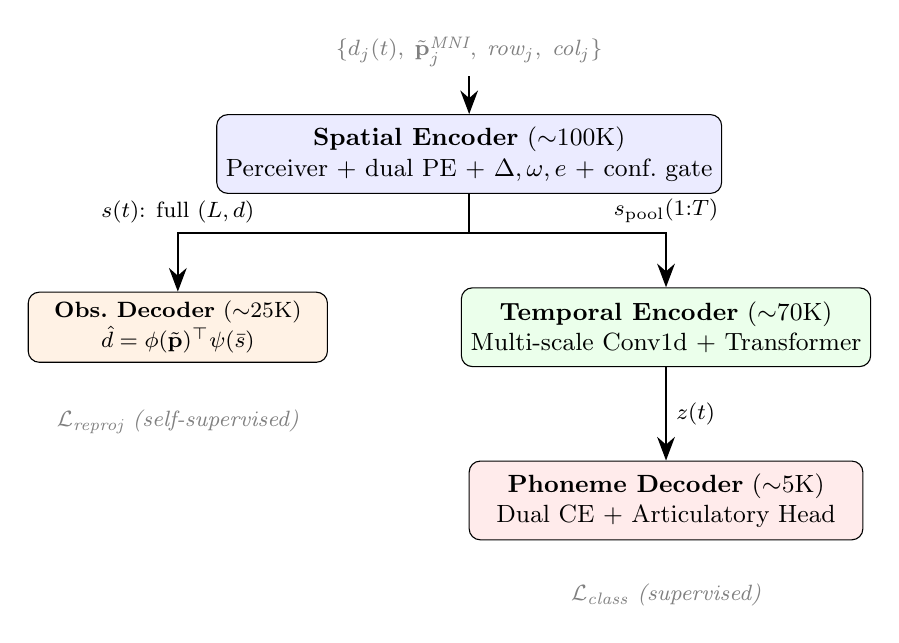
\begin{tikzpicture}[
  box/.style={draw, rounded corners, minimum width=5cm, minimum height=1cm, align=center, font=\small},
  smallbox/.style={draw, rounded corners, minimum width=3.8cm, minimum height=0.8cm, align=center, font=\footnotesize},
  arrow/.style={-{Stealth[length=3mm]}, thick},
  label/.style={font=\footnotesize\itshape, text=gray}
]

\node[box, fill=blue!8] (spatial) at (0, 0) {\textbf{Spatial Encoder} (${\sim}$100K)\\Perceiver + dual PE + $\Delta, \omega, e$ + conf.\ gate};

\node[smallbox, fill=orange!10] (obs) at (-3.7, -2.2) {\textbf{Obs.\ Decoder} (${\sim}$25K)\\$\hat{d} = \phi(\tilde{\bfp})^\top\psi(\bar{s})$};

\node[box, fill=green!8] (temporal) at (2.5, -2.2) {\textbf{Temporal Encoder} (${\sim}$70K)\\Multi-scale Conv1d + Transformer};

\node[box, fill=red!8] (phoneme) at (2.5, -4.4) {\textbf{Phoneme Decoder} (${\sim}$5K)\\Dual CE + Articulatory Head};

\node[label] (input) at (0, 1.3) {$\{d_j(t),\; \tilde{\bfp}_j^{\text{MNI}},\; \text{row}_j,\; \text{col}_j\}$};

\draw[arrow] (input) -- (spatial);
\draw[arrow] (spatial.south) -- ++(0,-0.5) -| (obs.north) node[midway, above, font=\footnotesize] {$s(t)$: full $(L,d)$};
\draw[arrow] (spatial.south) -- ++(0,-0.5) -| (temporal.north) node[midway, above, font=\footnotesize] {$s_{\text{pool}}(1{:}T)$};
\draw[arrow] (temporal) -- (phoneme) node[midway, right, font=\footnotesize] {$z(t)$};

\node[label] at (-3.7, -3.4) {$\mathcal{L}_{\text{reproj}}$ (self-supervised)};
\node[label] at (2.5, -5.6) {$\mathcal{L}_{\text{class}}$ (supervised)};

\end{tikzpicture}
\end{center}

\begin{equation}
\boxed{\mathcal{L} = \mathcal{L}_{\text{class}} + \lambda \cdot \mathcal{L}_{\text{reproj}}}
\end{equation}

\begin{table}[h]\centering\small
\begin{tabular}{@{}lrl@{}}
\toprule
\textbf{Module} & \textbf{Params} & \textbf{Role} \\
\midrule
Spatial encoder & ${\sim}$100K & Invert observation function \\
Observation decoder & ${\sim}$25K & Forward model (reprojection) \\
Temporal encoder & ${\sim}$70K & Dynamics modeling \\
Phoneme decoder & ${\sim}$5K & Classification \\
\midrule
\textbf{Total shared} & $\mathbf{{\sim}200}$\textbf{K} & \\
Per-patient ($\times 10$) & 700 & Registration + identity \\
\textbf{Grand total} & $\mathbf{{\sim}201}$\textbf{K} & (cf.\ current pipeline: 122K) \\
\bottomrule
\end{tabular}
\end{table}


%% ====================================================================
%%  PART IV: TRAINING, EVALUATION, AND EXPERIMENTAL DESIGN
%% ====================================================================

\part{Training, Evaluation, and Experimental Design}

\section{Training Pipeline}

\subsection{Phase 1: Source patient training (supervised + reprojection)}

9 source patients, ${\sim}1315$ labeled trials. Each batch:
\begin{enumerate}[leftmargin=2em]
\item \textbf{Spatial encoding}: construct tokens, mask 20--40\% electrodes, Perceiver $\to s(t)$, attention pooling $\to s_{\text{pool}}(t)$.
\item \textbf{Reprojection}: decoder predicts all electrodes (including masked) from $\bar{s}(t) = \text{mean}(s(t))$; compute $\mathcal{L}_{\text{reproj}}$ (or $\mathcal{L}_{\text{reproj}}^{\text{UQ}}$).
\item \textbf{Temporal encoding}: $s_{\text{pool}}(1{:}T) \to$ multi-scale $\to$ transformer $\to z(t)$.
\item \textbf{Classification}: dual head $\to \mathcal{L}_{\text{class}}$.
\item \textbf{Total}: $\mathcal{L} = \mathcal{L}_{\text{class}} + \lambda \mathcal{L}_{\text{reproj}}$ ($\lambda$: $0.5 \to 0.1$ annealed).
\end{enumerate}

\textbf{Optimizer}: AdamW with differential LR:
\begin{itemize}[leftmargin=2em]
\item Shared parameters: $10^{-3}$
\item Virtual positions, $\Delta$, $\omega$: $3 \times 10^{-4}$ (slow---geometric stability)
\item Patient $e$: $10^{-3}$
\end{itemize}

Linear warmup (20 epochs) $\to$ cosine decay. Weight decay $10^{-4}$. Gradient clipping 5.0. Batch size 16. Early stopping on held-out 20\% source validation, patience 7.

\subsection{Phase 2: Target adaptation (LP-FT)}

Per CV fold on target patient (5-fold grouped-by-token):
\begin{enumerate}[leftmargin=2em]
\item \textbf{Linear probe}: freeze encoder, train decoder + $\Delta^{(\text{target})} + \omega^{(\text{target})} + e^{(\text{target})}$. Initialize $e = \text{mean}(e^{(\text{source})})$. 150 epochs. Loss: $\mathcal{L}_{\text{class}} + 0.1 \cdot \mathcal{L}_{\text{reproj}}$.
\item \textbf{Fine-tune}: unfreeze encoder at $0.1\times$ LR. 100 epochs, patience 7.
\end{enumerate}

\subsection{Phase 3 (optional): Reprojection pre-training}

Pre-train spatial encoder + observation decoder on all available data using $\mathcal{L}_{\text{reproj}}$ only. No labels needed. Then initialize Phase~1 from pre-trained weights.


\section{Evaluation Protocol}

PER via edit distance, grouped-by-token 5-fold CV. Full recipe: weighted $k$-NN ($k{=}10$, cosine), TTA 16, dual head, best-of per fold, source $k$-NN at $0.5\times$ weight. Conformal prediction sets as interpretability output.


\section{Ablation Experiments}

\begin{table}[h]\centering\small
\begin{tabular}{@{}clp{7cm}@{}}
\toprule
\textbf{ID} & \textbf{Ablation} & \textbf{Question} \\
\midrule
A1 & MNI PE present/absent & \textbf{Central}: do MNI coordinates help? \\
 & \quad a. Current Conv2d + BiGRU baseline & $\to$ 0.762 \\
 & \quad b. Perceiver + Grid PE only & $\to$ architecture benefit \\
 & \quad c. Perceiver + MNI + Grid PE & $\to$ MNI benefit \\
 & \quad d. (c) + reprojection loss & $\to$ reprojection benefit \\
\midrule
A2 & \textbf{Population-level (all patients)} & \textbf{Is the 0.76 wall S14-specific?} \\
\midrule
A3 & Per-patient params & $\Delta$ only / $+\omega$ / $+e$ / position-dep.\ $e$ \\
A4 & Virtual electrode count & $L \in \{4, 8, 16, 32\}$ \\
A5 & Reprojection weight & $\lambda \in \{0, 0.01, 0.1, 0.5\}$ \\
A6 & Cross-task pooling & $+$ Duraivel data (architecture-independent) \\
A7 & Uncertainty stack & Beta-NLL + conf.\ gate vs.\ MSE-only \\
A8 & Spatial readout & MaxPool / attention pooling / full $(L,d)$ to temporal \\
A9 & Bilinear vs.\ MLP decoder & $\phi^\top\psi$ vs.\ $\text{MLP}([\tilde{\bfp}; e; \bar{s}])$ \\
A10 & Temporal backbone & Transformer vs.\ BiGRU (+ stride re-validation) \\
\bottomrule
\end{tabular}
\end{table}


\section{Experimental Priorities}\label{sec:priorities}

The document's own evidence suggests a clear priority ordering that should be stated transparently:

\begin{enumerate}[leftmargin=2em]
\item \textbf{Cross-task data pooling} (A6). Lowest risk, highest confidence. Same phonemes, overlapping patients, validated by Duraivel 2025. Directly addresses target-data scarcity. Can be tested with the current pipeline \textbf{and} the new architecture. Should be pursued first, in parallel with coordinate sourcing.

\item \textbf{Population-level evaluation} (A2). Pure methodology fix. Required to determine whether the 0.76 wall is S14-specific (55-experiment overfitting) or universal. Must be the \textbf{primary success criterion}, not just an ablation. Zero architectural risk.

\item \textbf{MNI coordinate-based architecture} (A1, this document). A working hypothesis. The evidence that spatial alignment is THE binding constraint is suggestive but unvalidated: it has not been isolated from data scarcity, measurement noise, or S14-specific effects (Section~\ref{sec:wall}). The architectural investment is justified by: (a)~MNI coordinates are currently unused information; (b)~the observation function formulation provides a principled framework; (c)~every component has a validated analog in 3D vision. But the hypothesis could be wrong---coordinates may not help if the wall is data-limited rather than alignment-limited.
\end{enumerate}

\textbf{The architecture is the most speculative of the three paths.} This is acceptable---it is the path with the most intellectual contribution if it works---but the document should not obscure the priority ordering.


\section{Success Criteria}\label{sec:success}

\textbf{Primary criterion (population-level):}
\begin{itemize}[leftmargin=2em]
\item Mean PER across all patients improves over current LOPO baseline with best architecture (A1c/d vs.\ A1a), evaluated across ${\geq}3$ seeds.
\item This is the only criterion that provides scientific evidence for the MNI coordinate hypothesis.
\end{itemize}

\textbf{Secondary criteria (S14 pilot---informative but not definitive):}
\begin{itemize}[leftmargin=2em]
\item A1c outperforms A1b by ${\geq}2\pp$ on S14 (MNI adds value beyond architecture change).
\item PER ${<}$ 0.740 on S14 (LOPO exceeds per-patient).
\end{itemize}

\caveat{S14 criteria are contaminated by 55+ prior experiments. Population-level results should take precedence if they disagree.}

\textbf{Interpretability (qualitative validation):}
\begin{itemize}[leftmargin=2em]
\item Virtual electrode positions cluster over known speech motor regions.
\item Learned $\Delta^{(i)}, \omega^{(i)}$ correlate with known registration quality (larger for tumor patients).
\item Spatial tuning vectors $\phi(\bfp)$ recover articulatory somatotopy when visualized.
\item Confidence gate $c_j$ correlates with electrode impedance or SNR.
\end{itemize}


\section{Available Data}

\begin{table}[h]\centering\small
\begin{tabular}{@{}lllc@{}}
\toprule
\textbf{Data source} & \textbf{Volume} & \textbf{Usage} & \textbf{Risk} \\
\midrule
PS task HGA & 9 pts, ${\sim}$1315 trials & Source training & -- \\
S14 HGA & 153 trials & Target evaluation & -- \\
Cross-task (Duraivel) & 3 pts, 156--208 trials & \textbf{Priority 1: more data} & Low \\
MNI coordinates & All patients & Perceiver architecture & Medium \\
Continuous recordings & ${\sim}168$\,min & Phase 3 reprojection SSL & Medium \\
Lexical task patients & 13 patients & Additional sources & Medium \\
\bottomrule
\end{tabular}
\end{table}


\section{MNI Coordinate Sourcing}

Hard dependency. Likely locations: BioImage Suite outputs (DBS), Brainlab (tumor), ECoG\_Recon on Box. Fallback: scaled ACPC grid positions (retains within-patient structure, loses cross-patient alignment).


\section{Risk Assessment}

\begin{table}[h]\centering\small
\begin{tabular}{@{}p{0.33\textwidth}cp{0.44\textwidth}@{}}
\toprule
\textbf{Risk} & \textbf{Sev.} & \textbf{Mitigation} \\
\midrule
MNI coordinates unavailable & High & Fallback to Grid PE only \\
MNI alignment too imprecise & High & Ablation A1; learnable $\alpha$ adapts blur \\
Reprojection competes with classification & Medium & $\lambda$ ablation A5; $\lambda{=}0$ fallback \\
Perceiver overfits (200K, 1300 trials) & Medium & Masking; early stopping; reprojection reg. \\
Bilinear separability too restrictive & Medium & Ablation A9: MLP fallback \\
Per-patient params insufficient for tumor distortion & Medium & Ablation A3; position-dep.\ $e$ option \\
Virtual electrodes collapse & Low & Initialize across convex hull; monitor \\
\bottomrule
\end{tabular}
\end{table}


\section{Summary}

This document formalizes cross-patient speech decoding as \textbf{multi-view neural field reconstruction} with explicit acknowledgment of where the analogy holds and where it breaks (Section~\ref{sec:disanalogies}).

The architecture produces two distinct representations: $s(t)$ (per-frame spatial summary, trained via reprojection) and $\bfz(t)$ (temporally-refined state, trained via classification). The observation decoder uses a bilinear factorization that assumes separability between spatial tuning and articulatory activation---a structural hypothesis validated in physical field reconstruction but unverified for coarticulatory neural dynamics (ablation A9).

Key improvements over v2: (1)~explicit $s(t)$ vs.\ $\bfz(t)$ distinction resolving the theory-architecture mismatch; (2)~attention-based readout replacing MaxPool to preserve somatotopic decomposition; (3)~per-patient rotation $\omega^{(i)}$ alongside translation $\Delta^{(i)}$; (4)~mechanically specified uncertainty connection (confidence gate $c_j$ on attention values, Beta-NLL on reprojection loss); (5)~honest acknowledgment of the bilinear separability assumption; (6)~``where the analogy breaks'' section; (7)~population-level as primary success criterion; (8)~transparent experimental priority ordering (data $>$ population eval $>$ architecture); (9)~expanded ablation plan (A1--A10); (10)~flagged assumptions in red throughout.

Total budget: ${\sim}200$K shared + 70 per patient. Every component maps to the observation equation, with structural assumptions explicitly marked for empirical validation.

\end{document}
